\section{Framebuffer DMA processor}
\label{sec:framebuffer_dma}

\begin{figure}
  \centering
  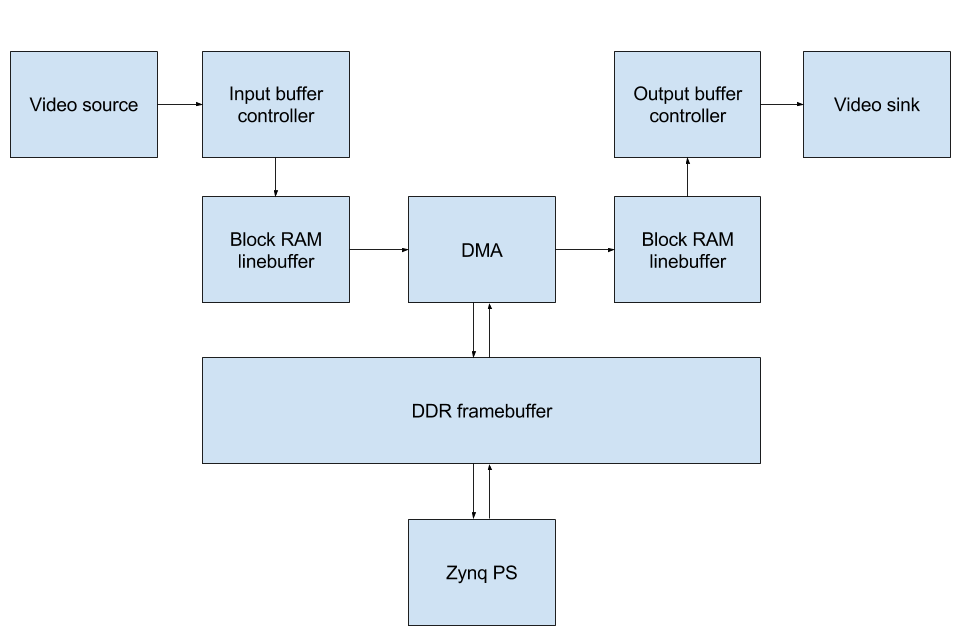
\includegraphics[width=1\textwidth]{./img/framebuffer_block_diagram.png}
  \caption{Block diagram of the framebuffer DMA processor. Image data is stored in a temporary input before being copied to the main framebuffer. A similar configuration on the output allows image data to be modified by the Zynq PS and transmitted.}
  \label{fig:dma_endianness}
\end{figure}

A framebuffer is a portion of memory which holds the current frame, allowing the hardware blocks either side to act in complete isolation. Both sides of the link use framebuffers, though their purpose differs. On the receiver side the framebuffer stores each frame before it is written to flash storage. Firmware inside the Zynq \gls{ps} \marginpar{Explain the Zynq PS} can draw to the frame in real-time, adding helpful indicators such as the currently connected sensor module and gridlines to aid the photographer's composition process. On the transmitter side the framebuffer serves a different purpose. A critical flaw in the design of the \gls{dvi} receiver causes the link to break if the incoming pixel clock is less than \SI{40}{\mega\hertz} --- a potential issue because the OV7670's pixel clock is only \SI{12}{\mega\hertz}. To mitigate this, the transmitter sends out duplicate frames, thus bringing the pixel clock up into the region required for correct operation.

The space required to store frames is a direct function of the image resolution. As the OV7670 outputs frames in 640 x 480 resolution, a \SI{307.2}{\kilo\byte} framebuffer is required. While \glspl{fpga} usually contain a small amount of internal block RAM, there is insufficient space for storing an entire frame. Though its access is significantly more complicated, the Zynq-7000 includes a hard DDR controller which can be utilised to store the frames in external DDR3 memory instead --- the Zybo development board contains \SI{512}{\mega\byte} of RAM, which is more than sufficient for storing a single frame.

\marginpar{Diagram of internal Zynq arch - access to DDR}

\subsection{AXI}
Due to the internal architecture of the Zynq-7000, external RAM is only accessible from the \gls{ps}, thus incoming frames which are processed by the \gls{pl} must be fed into the \gls{ps} before they can be stored in the RAM. Fortunately the \gls{pl} and \gls{ps} are able to exchange data using the \gls{axi} interface, which was designed to provide a single interconnect for IP across all domains. While there are several different variants of \gls{axi} (a comparison of which is found in Table \ref{table:axi_comparison}), they all operate in fundamentally the same way. \gls{axi} is used to connect a master device to a slave device using one or more channels which are used to carry out transactions. A standard AXI4 connection will consist of five channels:
\begin{itemize}
  \item Read Address Channel
  \item Write Address Channel
  \item Read Data Channel
  \item Write Data Channel
  \item Write Response Channel
\end{itemize}
(\url{http://www.xilinx.com/support/documentation/ip_documentation/axi_ref_guide/latest/ug1037-vivado-axi-reference-guide.pdf})

\begin{table}[]
\centering
\caption{Comparison of AXI interfaces. Adapted from (\url{http://www.xilinx.com/support/documentation/ip_documentation/axi_ref_guide/latest/ug1037-vivado-axi-reference-guide.pdf}).}
\label{table:axi_comparison}
\begin{tabular}{llll}
              & AXI4                               & AXI4-Lite                      & AXI4-Stream                \\
Dedicated for & High-performance and memory-mapped & Register-style interfaces      & Non-address based IP       \\
Burst         & Up to 256                          & 1                              & Unlimited                  \\
Data width    & 32 - 1024 bits                     & 32 / 64 bits                   & Anything                   \\
Applications  & Embedded, memory                   & Small footprint logic, control & DSP, video, communications
\end{tabular}
\end{table}

As separate channels are used for reading and writing, device communication is fully bi-directional. In addition to the address and data signals, extra signals are provided for control and synchronisation to ensure that a device can only begin a transaction when the other device is ready. Figure \ref{fig:axi_architecture} illustrates a typical AXI4 interface. 

\begin{figure}
\centering
\begin{subfigure}{.5\textwidth}
  \centering
  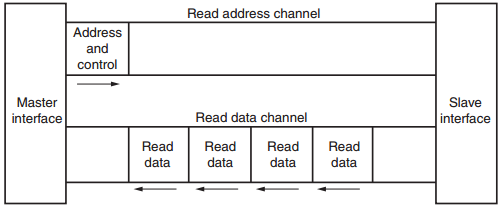
\includegraphics[width=.4\linewidth]{./img/axi_read.png}
  \caption{Read Channel}
\end{subfigure}%
\begin{subfigure}{.5\textwidth}
  \centering
  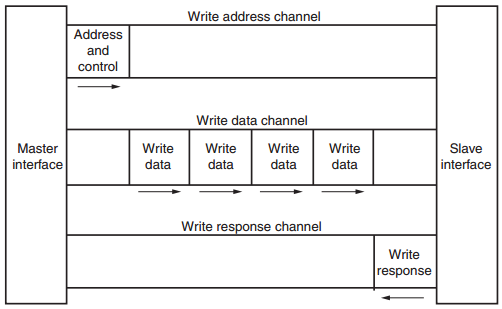
\includegraphics[width=.4\linewidth]{./img/axi_write.png}
  \caption{Write Channel}
\end{subfigure}
\caption{Architecture of AXI4 Read and Write Channels. (\url{http://www.xilinx.com/support/documentation/ip_documentation/axi_ref_guide/latest/ug1037-vivado-axi-reference-guide.pdf})}
\label{fig:axi_architecture}
\end{figure}

All hardware inside the Zynq can be addressed from the \gls{ps} provided it has been connected via \gls{axi}. AXI requires all devices to be assigned an address which complies with the address map in Table \ref{table:zynq_address_map}. For example, the \gls{axi} master port \texttt{M\_AXI\_GP0} on the \gls{ps} has the address range \texttt{0x4000\_0000} to \texttt{0x7FFF\_FFFF}. Any \gls{axi} slave devices in the \gls{pl} assigned an address in this range can be accessed from the \gls{ps}. Conversely, any \gls{axi} master devices in the \gls{pl} connected to the \gls{ps} slave port \texttt{S\_AXI\_HP0} can access most of the DDR address range.

\begin{table}[]
\centering
\caption{Zynq-7000 system-level address map. (\url{http://www.xilinx.com/support/documentation/user_guides/ug585-Zynq-7000-TRM.pdf})}
\label{table:zynq_address_map}
\begin{tabular}{lllll}
Address range                             & CPUs and ACP & AXI\_HP & Other bus masters & Notes                                                 \\
\multirow{4}{*}{0000\_0000 to 0003\_FFFF} & OCM          & OCM     & OCM               & Address not filtered by SCU and OCM is mapped low     \\
                                          & DDR          & OCM     & OCM               & Address filtered by SCU and OCM is mapped low         \\
                                          & DDR          &         &                   & Address filtered by SCU and OCM is not mapped low     \\
                                          &              &         &                   & Address not filtered by SCU and OCM is not mapped low \\
\multirow{2}{*}{0004\_0000 to 0007\_FFFF} & DDR          &         &                   & Address filtered by SCU                               \\
                                          &              &         &                   & Address not filtered by SCU                           \\
\multirow{2}{*}{0008\_0000 to 000F\_FFFF} & DDR          & DDR     & DDR               & Address filtered by SCU                               \\
                                          &              & DDR     & DDR               & Address not filtered by SCU                           \\
0010\_0000 to 3FFF\_FFFF                  & DDR          & DDR     & DDR               & Accessible to all interconnect masters                \\
4000\_0000 to 7FFF\_FFFF                  & PL           &         & PL                & General Purpose Port \#0 to the PL, M\_AXI\_GP0       \\
8000\_0000 to BFFF\_FFFF                  & PL           &         & PL                & General Purpose Port \#1 to the PL, M\_AXI\_GP1       \\
E000\_0000 to E02F\_FFFF                  & IOP          &         & IOP               & I/O Peripheral registers                              \\
E100\_0000 to E5FF\_FFFF                  & SMC          &         & SMC               & SMC Memories                                          \\
F800\_0000 to F800\_0BFF                  & SLCR         &         & SLCR              & SLCR registers                                        \\
F800\_1000 to F880\_FFFF                  & PS           &         & PS                & PS System registers                                   \\
F890\_0000 to F8F0\_2FFF                  & CPU          &         &                   & CPU Private registers                                 \\
FC00\_0000 to FDFF\_FFFF                  & Quad-SPI     &         & Quad-SPI          & Quad-SPI linear address for linear mode               \\
\multirow{2}{*}{FFFC\_0000 to FFFF\_FFFF} & OCM          & OCM     & OCM               & OCM is mapped high                                    \\
                                          &              &         &                   & OCM is not mapped high                               
\end{tabular}
\end{table}

\subsection{Linebuffers}
Due to the high complexity of the DDR controller, memory operations are not instantaneous and have non-deterministic latencies, thus an additional buffer must be placed between the incoming frames from the \texttt{ov7670\_capture} block and framebuffer, and a second between the framebuffer and the \texttt{rgb2dvi} module.

Each line of the input frame is written into a \SI{2048}{\kilo\bit} linebuffer pixel-by-pixel. The block RAM for each linebuffer can either be configured in standalone mode or for use with an AXI BRAM Controller instance. The block RAM has its own address space (starting at \texttt{0x0000} up to however large the block RAM is), and so an AXI BRAM Controller instance is placed between the block RAM and input AXI CDMA instance (\texttt{i\_axi\_cdma}) to translate between the two address spaces. As the block RAM is operating in BRAM Controller mode the following Block Memory Generator configuration is used:
\begin{itemize}
  \item 32-bit data width
  \item 2048-bit data depth
  \item 32-bit address width
  \item Byte addressing
\end{itemize}

\subsection{\texttt{i\_buf\_controller} module}
The \texttt{i\_buf\_controller} module is a simple shim which writes each line of the video into the linebuffer and triggers interrupts on the \gls{ps} to initiate a \gls{dma} transfer into the DDR framebuffer. Upon detecting the \texttt{vde} signal going high, the input buffer controller starts writing each incoming pixel into the linebuffer. Due to the 32-bit data width, each block RAM write consists of four 8-bit pixels packed together. Attention must be paid to the endianness when packing pixel data. Figure \ref{fig:dma_endianness} illustrates how packing the pixels into a 32-bit block will cause their order to become reversed when transferred as a result of little-endian storing the least significant bit in the lowest memory address. To ensure pixels are stored in the correct order in the DDR framebuffer they are shifted into a 32-bit shift register, with the left-most pixel stored as the least significant bits.

\begin{figure}
  \centering
  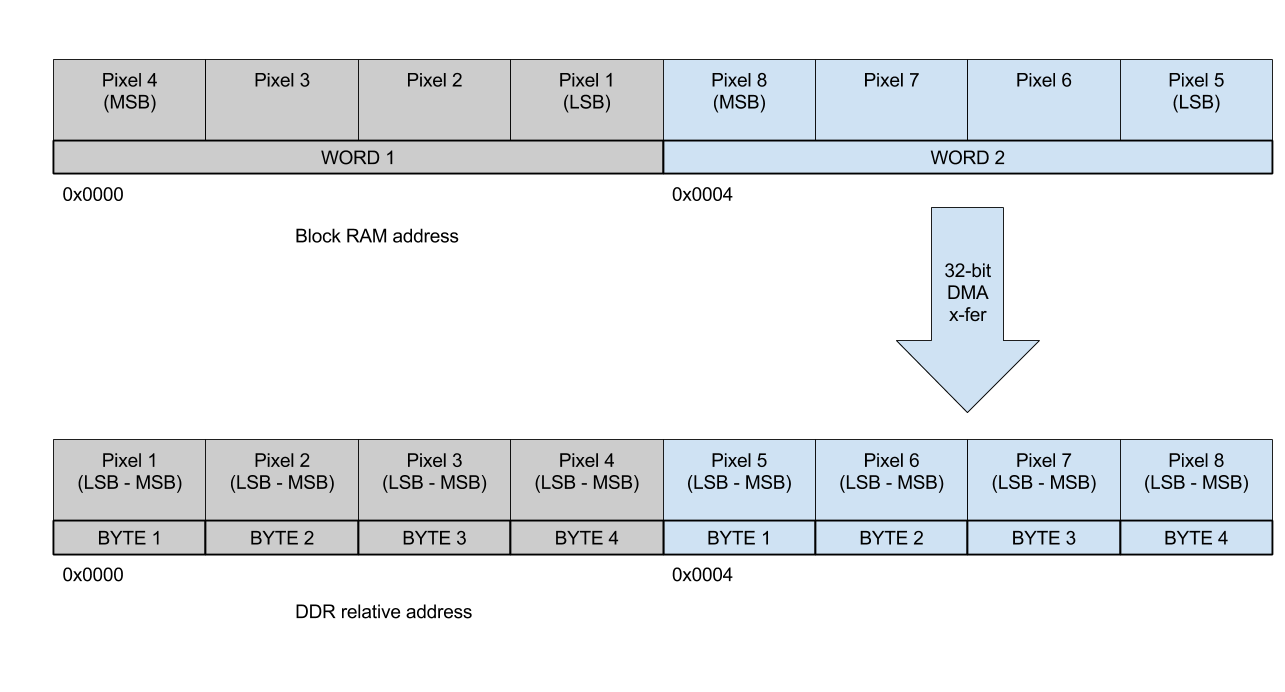
\includegraphics[width=1\textwidth]{./img/dma_endianness.png}
  \caption{32-bit DMA transfer of a block of four 8-bit pixels causes the pixel order to be reversed due to the little-endian architecture of the Zynq \gls{ps}.}
  \label{fig:dma_endianness}
\end{figure}

The blanking period provides a short interval during which the current linebuffer is transferred into the framebuffer by the \texttt{i\_axi\_cdma} instance. As any AXI CDMA transactions must be initiated from the \gls{ps}, the input buffer controller is connected to the \gls{ps} via two interrupt lines. As soon the last pixel in the line is written to the linebuffer, the input buffer controller triggers the \texttt{line\_valid} interrupt to notify the firmware running inside the \gls{ps} that it needs to copy the line into the main framebuffer. Similarly, the \texttt{frame\_valid} interrupt is triggered when the \texttt{vsync} signal is received, indicating a boundary between frames. The address generation and data packing logic is shown in Listing \ref{lst:i_buf_controller}.

\begin{lstlisting}[caption={Address generation and data packing logic for input framebuffer.}, label={lst:i_buf_controller}, language=Verilog]
// Latch data and address into BRAM
if (vde) begin
    h_count_stop <= h_count + 2;
    if (h_count < h_count_stop) begin
        h_count <= h_count + 1;
        o_data <= {i_data, o_data[31:8]};
        addr <= next_addr;
        we <= 0;
        if (!((h_count+1) % 4)) begin
            next_addr <= next_addr + 4;
            we <= 1;
        end
    end
end
\end{lstlisting}

\subsection{AXI CDMA and buffer control firmware}
Interrupts from the input and output buffer controllers are connected to the \gls{gic} on the \gls{ps} via the \texttt{IRQ\_F2P} line. Each interrupt connected to the \gls{gic} must be initialised individually. To help with this, the function in Listing \ref{lst:interrupt_setup} is used to connect each interrupt to an \gls{isr} and configure it to only trigger on the rising edge. Listing \ref{lst:isr_functions} show the four \glspl{isr} which handle the input and output buffer controller interrupts. \glspl{isr} should generally be kept as short as possible, and so flags are used to indicate to the main loop that a memory transaction is required.

\begin{lstlisting}[caption=[Interrupt setup function], label={lst:interrupt_setup}, language=C]
int create_interrupt(XScuGic *instance_p, u32 int_id, u8 priority, u8 trigger, Xil_InterruptHandler isr, void *callback_ref) {
    int status;

    // Connect interrupt controller hardware driver
    status = XScuGic_Connect(instance_p, int_id, isr, callback_ref);
    if (status != XST_SUCCESS) {
        return XST_FAILURE;
    }

    XScuGic_SetPriorityTriggerType(instance_p, int_id, priority, trigger);

    XScuGic_Enable(instance_p, int_id);

    return XST_SUCCESS;
}
\end{lstlisting}

\begin{lstlisting}[caption={\glspl{isr} for handling buffer controller interrupts.}, label={lst:isr_functions} language=C]
void line_valid_isr(void *line_valid_flag) {
    *((int *)line_valid_flag) = 1;
}

void frame_valid_isr(void *frame_valid_flag) {
  *((int *)frame_valid_flag) = 1;
}

void req_line_isr(void *req_line_flag) {
  *((int *)req_line_flag) = 1;
}

void req_frame_isr(void *req_frame_flag) {
  *((int *)req_frame_flag) = 1;
}
\end{lstlisting}

In order to deal with the high throughput, the Zynq \gls{ps} offloads large memory transfers to the dedicated \gls{dma} engine. Once the transfer has been initiated the \gls{ps} can return back to normal code execution, resulting in a much smaller overhead for memory transfers. The AXI Central DMA core can provide \gls{dma} transfers between connected AXI-compatible blocks. In this case two AXI CDMA instances are created: the \texttt{i\_axi\_cdma} instance is used to transfer data from the input linebuffer into the framebuffer, and the \texttt{o\_axi\_cdma} instace is used to transfer data from the framebuffer into the output linebuffer. In both cases the AXI CDMA master ports are connected to a high-performance AXI slave port on the \gls{ps} (giving high-speed access to the DDR RAM) and the input or output linebuffer via an AXI Block RAM Controller. These connections are illustrated in Figure \ref{fig:axi_cdma}.

\begin{figure}
  \centering
  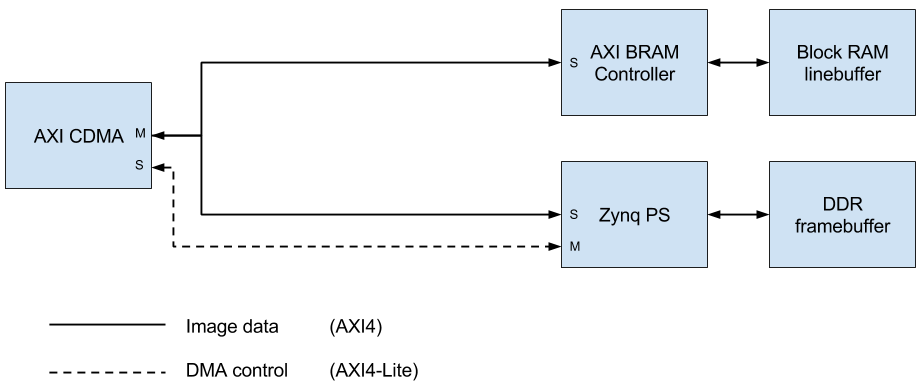
\includegraphics[width=1\textwidth]{./img/axi_cdma.png}
  \caption{Master ports of AXI CDMA instance are connected to Zynq PS for framebuffer access, and AXI BRAM Controller for linebuffer access. An additional AXI4-Lite interface allows control from the PS.}
  \label{fig:axi_cdma}
\end{figure}

The AXI CDMA core provides a control interface on its slave port. When connected to the \gls{ps}, the AXI CDMA exposes a set of control registers which can be used by the firmware is able to initiate \gls{dma} transfers. The key registers are (\url{http://www.xilinx.com/support/documentation/ip_documentation/axi_cdma/v4_1/pg034-axi-cdma.pdf}):
\begin{itemize}
  \item \texttt{SRCADDR}: Source address to transfer bytes from
  \item \texttt{DSTADDR}: Destination address to transfer bytes to 
  \item \texttt{BTT}: Number of bytes to transfer
\end{itemize}

Rather than write to these registers directly, the firmware uses a set of wrapper functions which perform various additional validation checks. Listing \ref{lst:update_buf_controller} details the buffer update routie which checks if any flags have been set by the \glspl{isr} in Listing \ref{lst:isr_functions}. When the \texttt{line\_valid} flag is set, the input buffer controller is indicating that the linebuffer is full and the \gls{ps} should copy it into the main framebuffer. Conversely, when the \texttt{req\_line} flag is set, the output buffer controller is indicating that it requires the \gls{ps} to copy a new line into the linebuffer. Should one of the line valid / line request flags be set, the firmware calls the \texttt{XAxiCdma\_SimpleTransfer()} function with the corresponding source address and destination address. This function sets the AXI CDMA control registers accordingly and then initiates the \gls{dma} transfer by writing to the \texttt{BTT} register. The firmware uses two pointers to keep track of memory offsets and ensure the correct line is written or copied from the two linebuffers. To improve performance, the \gls{ps} ARM core includes a data cache which helps avoid expensive external memory operations by storing commonly-accessed data in faster on-chip memory. Before initiating a \gls{dma} transfer the data cache needs to be wiped using the \texttt{Xil\_DCacheInvalidateRange()} and \texttt{Xil\_DCacheFlushRange()} functions, to prevent any stale data being transferred.

\begin{lstlisting}[caption={Buffer controller update loop}, label={lst:update_buf_controller}, language=C]
void update_buf_controller(void) {
    // Check the flags for transfers and address reset
    if (line_valid_flag) {
      // Cache flush is essential!!!
      Xil_DCacheInvalidateRange((UINTPTR)&g_framebuf[i_framebuf_line][0], FRAMEBUF_WIDTH);
        XAxiCdma_SimpleTransfer(&i_cdma, (UINTPTR)I_BRAM_AXI_ADDR, (UINTPTR)&g_framebuf[i_framebuf_line][0], FRAMEBUF_WIDTH, NULL, NULL);
        i_framebuf_line++;
        line_valid_flag = 0;
    }

    if (frame_valid_flag) {
        i_framebuf_line = 0;
        frame_valid_flag = 0;
    }

    if (req_line_flag) {
      Xil_DCacheFlushRange((UINTPTR)&g_framebuf[o_framebuf_line][0], FRAMEBUF_WIDTH);
      XAxiCdma_SimpleTransfer(&o_cdma, (UINTPTR)&g_framebuf[o_framebuf_line][0], (UINTPTR)O_BRAM_AXI_ADDR, FRAMEBUF_WIDTH, NULL, NULL);
      o_framebuf_line++;
      req_line_flag = 0;
    }

    if (req_frame_flag) {
        o_framebuf_line = 0;
        req_frame_flag = 0;
    }
} 
\end{lstlisting}

The frame valid / frame requests flags are simply used to reset the framebuffer pointer to the first line, meaning that the framebuffer is overwritten every frame. In a proper implementation, double or triple buffering would be used to ensure that the input linebuffer could not overwrite the frame currently being output, however this would have added unnecessary complexity to the design.


\marginpar{Include address map of relevant parts}

\marginpar{Diagram of OV7670 -> framebuffer -> DVI isolation, and DVI -> framebuffer -> SD / screen}

\subsection{\texttt{o\_buf\_controller} module}
\marginpar{Include portmap of module}
The output buffer controller is fundamentally the same as the input buffer controller, except its operation is reversed. The \texttt{o\_buf\_controller} module uses two interrupts, \texttt{req\_line} and \texttt{req\_frame}, to signal when the output linebuffer needs filling with the next line from the framebuffer.

As the data is read line-by-line, the output buffer controller generates the appropriate video timing signals (\texttt{vsync}, \texttt{hsync} and \texttt{vde}) which accompany the output pixel data \texttt{o\_data}. Because the vertical and horizontal synchronisation signals are entirely dependent on the video resolution, the module includes a set of user-configurable parameters. These parameters are used in Listing \ref{lst:o_buf_controller_vga_sync} to control the timing of the synchronisation pulses.

\begin{lstlisting}[caption={Output buffer controller video synchronisation generation logic.}, label={lst:o_buf_controller_vga_sync}, language=Verilog]
// VGA sync logic
// All of these have a 1-cycle delay to sync them with data output
vsync_next <= (v_count < (DISPLAY_HEIGHT + V_FRONT_PORCH)) ||
    (v_count >= (MAX_V_COUNT - V_BACK_PORCH));
vsync <= vsync_next;
hsync_next <= (h_count < (DISPLAY_WIDTH + H_FRONT_PORCH)) ||
    (h_count >= (MAX_H_COUNT - H_BACK_PORCH));
hsync <= hsync_next;
vde_next <= h_count < DISPLAY_WIDTH-1 && v_count < DISPLAY_HEIGHT;
vde <= vde_next;
\end{lstlisting}

Much like the input buffer controller, the block RAM has a 32-bit wide data interface, thus the pixels are transferred in blocks of four and need to be unpacked and re-ordered before they can be output. The code in Listing \ref{lst:data_unpacking} performs the address generation and data unpacking.

\begin{lstlisting}[caption={Address generation and data unpacking logic for output buffer controller.}, label={lst:data_unpacking}, language=Verilog]
h_count <= h_count + 1;
o_data <= (i_data >> (((h_count) % 4) * 8)) & 'h000000ff;
if (h_count < DISPLAY_WIDTH-1) begin
    if (!((h_count+2) % 4) ) begin
        addr <= addr + 4;
    end
end else begin
    addr <= 0;
end
\end{lstlisting}